\section{Experimental Evaluation}
\label{sec:evaluation}

We evaluate \Treebeard{} on two machines. The first one has an Intel Core
i9-11900K (Rocket Lake) processor with 8 physical cores (16 logical cores with
hyperthreading), 128~GB of RAM and Ubuntu~20.04.3 LTS.  The second system has an
AMD Ryzen~7 4700G process with 8 physical cores (16 logical cores with
hyperthreading), 64~GB of RAM, and runs CentOS Linux release 7.9.2009. For
comparisons with XGBoost and Treelite, we used Python version 3.10, XGBoost
version 1.5.0 and Treelite version 2.3.0.

% Linux kernel version 5.11.0.

The benchmark models we used are trained using datasets listed in Table~\ref{Tab:Benchmarks}. These datasets were also used by the Intel Machine Learning
Benchmark suite~\cite{MLBenchmarks}. We used
the hyper-parameters from this suite for all the datasets. All models were trained
with XGBoost~\cite{XGBoost}.  For all experiments, we run inference on 2 million test
inputs (divided into the required number of batches). To compute speedups, we
compare the mean time taken per input row between configurations.

\begin{table}
  \centering
  \small{
  \begin{tabularx}{\linewidth}{c r r r r}
   \toprule
   \textbf{Dataset} & \textbf{\#Features} & \textbf{\#Trees} & \textbf{Max Depth} & \textbf{\#Leaf-biased}\\
   \midrule
   \texttt{abalone} & 8 & 1000 & 7 & 438\\
   \texttt{airline} & 13 & 100 & 9 & 8 \\
   \texttt{airline-ohe} & 692 & 1000 & 9 & 976 \\
   \texttt{covtype} & 54 & 800 & 9 & 283\\
   \texttt{epsilon} & 2000 & 100 & 9 & 0\\
   \texttt{letter} & 16 & 2600 & 7 & 0 \\
   \texttt{higgs} & 28 & 100 & 9 & 8\\
   \texttt{year} & 90 & 100 & 9 & 0\\
   \bottomrule
  \end{tabularx}
  \vskip 5pt
  \caption{\label{Tab:Benchmarks}List of benchmark datasets and their 
  parameters. 
  The column \op{Leaf-biased} reports the number of leaf-biased trees per benchmark with $\langle\alpha =0.075, \beta =0.9 \rangle$ . }
  }
\end{table}

%\TODO{AP How do we say that we tried several optimizations and picked the best?}
In order to find the best combination of optimizations, several configurations were explored
for each benchmark at different batch sizes. The grid of optimizations explored is listed in Table~\ref{Tab:Optimizations}. 
%% RG
We report performance results for inference performed using (i) \Treebeard{} baseline code without performing any optimizations
presented in Sections~\ref{Sec:HIR}, \ref{Sec:MIR} and \ref{Sec:LIR}, (ii) \Treebeard{} code with the combination of optimizations that performs best,
(iii) XGBoost, and (iv) Treelite. We refer to the unoptimized \Treebeard{} code as the scalar baseline.
% \begin{enumerate}
%   \item \emph{Loop order} : One tree at a time vs. one row at a time
%   \item \emph{Tile size} : 1, 2, 4, 8
%   \item \emph{Tiling type} : Basic tiling vs probability-based tiling
%   \item \emph{Tree padding and unrolling} : Yes or no
%   \item \emph{Tree walk interleaving} : 2, 4, 8 (Number of walks interleaved)
% \end{enumerate}
\begin{table}[htbp]
  \small{
  \begin{tabularx}{\linewidth}{l l}
   \toprule
   \textbf{Optimization} & \textbf{Configurations}\\
   \midrule
   \multirow{2}{*}{\texttt{Loop order}} &  One tree at a time\\
                       &  One row at a time\\
   \midrule
   \texttt{Tile size} & 1, 2, 4, 8 \\
   \midrule
   \multirow{2}{*}{\texttt{Tiling type}} & Basic tiling\\
   & Probability-based tiling \\
   \midrule
   \texttt{Tree padding and unrolling} & Yes, No \\
   \midrule
   \texttt{Tree walk interleaving} & 2, 4, 8 \\
   \midrule
   \texttt{$\langle \alpha, \beta\rangle$ for leaf-bias} &  $\langle0.05, 0.9 \rangle$, $\langle0.075, 0.9 \rangle$ , $\langle 0.1, 0.9 \rangle$ \\
     \bottomrule
  \end{tabularx}
  \vskip 5pt
  \caption{\label{Tab:Optimizations}Space of optimizations explored.}
  }
\end{table}
\CommentOut{
\TODO{kr: this is out of place. Future work?}
Even though \Treebeard{} has the ability to perform non-trivial rewrites of the loop nest over
tree, input row pairs, we do not explore anything beyond the simple loop interchange listed above
in the current work. We leave a more thorough exploration of loop optimizations to future work.
}
% \subsection{Outline}
% \begin{enumerate}
%   \item Summary plot -- speedups over unopt baseline for both Intel and AMD. One bar graph for specific batch size over all benchmarks + geo mean. (AMD + Intel)
%   \item Effectiveness of optimizations (AMD + Intel)
%   \begin{enumerate}
%     \item Speedup with basic + prob tiling
%     \item Speedup with unroll etc etc
%   \end{enumerate}
%   \item Parallel scaling
%   \begin{enumerate}
%     \item Speedup over batch sizes with all cores -- one line plot and one bar graph for a specific batch size (Intel + AMD)
%     \item Mean speedup scaling with number of cores (Intel + AMD)
%   \end{enumerate}
%   \item Speedup over xgboost and treelite (intel only) -- parallel and serial. For each, one line graph and one bar graph.
% \end{enumerate}

% \begin{figure}
%   \centering
%   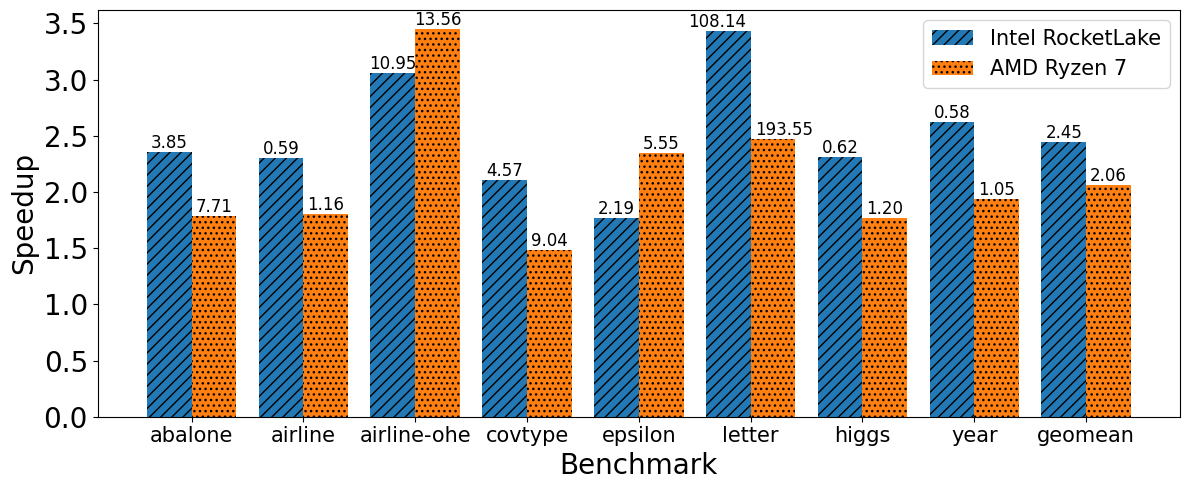
\includegraphics[width=\linewidth]{figures/result/scalar_overall_speedup_benchmark_intel_amd.png}
%   \caption{Overall single-core speedup of optimized \Treebeard{} code over a na\"ive scalar baseline at batch size of 1024.}
%   \label{Fig:OverallScalar}
% \end{figure}

% \begin{figure}
%   \centering
%   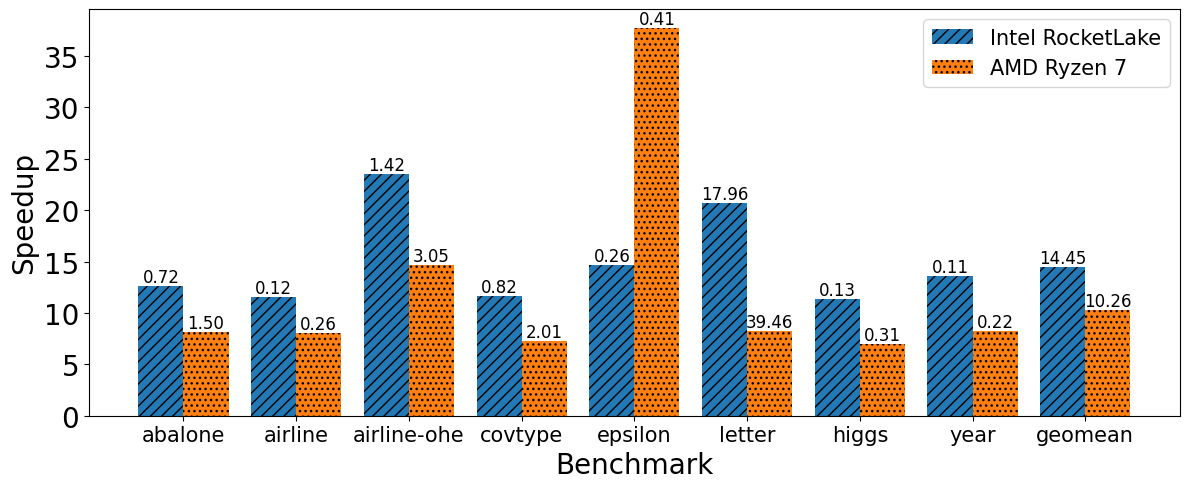
\includegraphics[width=\linewidth]{figures/result/parallel_overall_speedup_benchmark_intel_amd.png}
%   \caption{Overall multi-core speedup of optimized \Treebeard{} code over a na\"ive scalar baseline at batch size of 1024 and with 16 cores.}
%   \label{Fig:OverallParallel}
% \end{figure}

\begin{figure*}[tbp]
  \centering
  \subfloat[Single-core]{
    \centering
    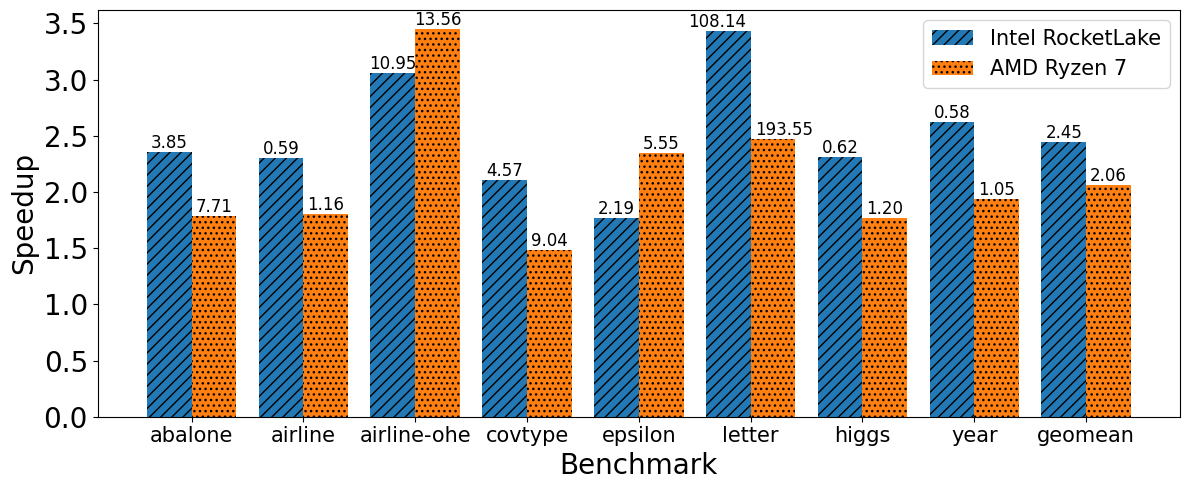
\includegraphics[width=0.48\linewidth]{figures/result/scalar_overall_speedup_benchmark_intel_amd.png}
    \label{Fig:OverallScalar}
  }
  \subfloat[16 cores]{
    \centering
    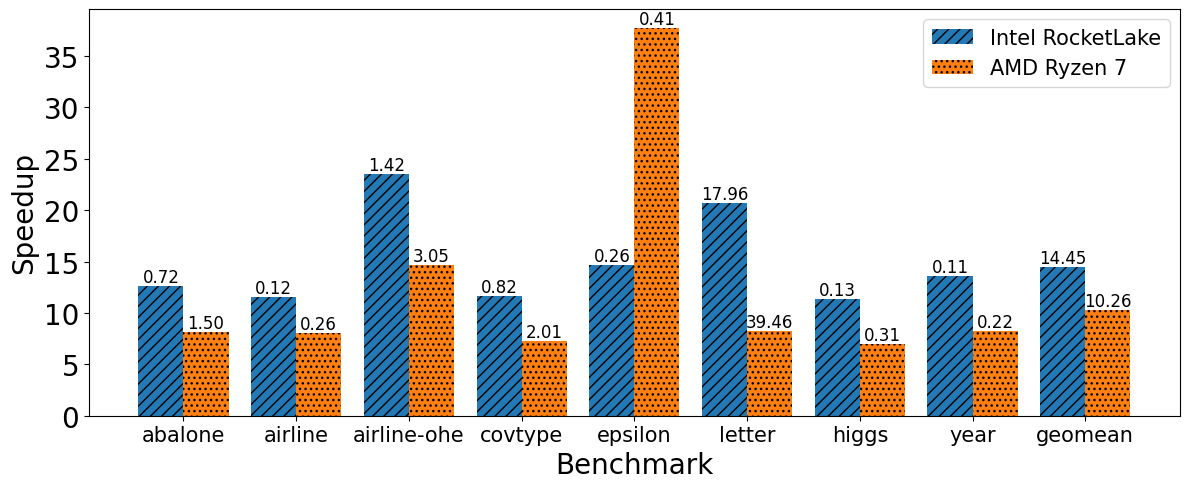
\includegraphics[width=0.48\linewidth]{figures/result/parallel_overall_speedup_benchmark_intel_amd.png}
    \label{Fig:OverallParallel}
  }
  \caption{Speedup of \Treebeard{} optimized code over the scalar baseline 
           at batch size of 1024. Number over each bar is the mean time to 
           perform inference on one input row in $\mu$s. Numbers on the geomean bars 
           are the geomean speedups over all benchmarks.}
  \label{fig:Summary}
\end{figure*}

\subsection{Summary of Improvements on Different Hardware}
Figure~\ref{Fig:OverallScalar} compares the single core performance of \Treebeard{} optimized code with the scalar baseline, on different hardware. The plot has two bars corresponding to the Intel and AMD machines,
each showing the speedup of the optimized version over the corresponding baseline.
As can be seen, \Treebeard{} does consistently better on all benchmarks, attaining up to $3.5\times$ speedup on both machines.
Between Intel and AMD we find that on average the speedups are a little better on Intel. This is because the Intel machine has a much
more efficient implementation of the \op{gather} instruction. Our vectorized implementation uses this to load features.
Because of this and other differences in low level architecture we find that the best set of optimizations on the two machines are completely different. On the
Intel machine we aggressively tile the tree with a tile size of 8 for all benchmarks. While on the AMD machine optimal
performance is sometimes achieved at much lower tile sizes (\op{airline} prefers a tile size of 1,
\op{airline-ohe}, \op{covtype} and \op{epsilon} prefer a tile size of 4). Similarly, we interleave walks more aggressively
on Intel than on AMD, interleaving by a factor of eight works best on the Intel
system on all benchmarks, while on the AMD one, two benchmarks perform optimally
with an interleaving of four.

Figure~\ref{Fig:OverallParallel} compares multi-core performance with 16 cores on different hardware. All speedups are
reported with respected to an unoptimized single core run. As can be seen even with simple parallelization 
we are able to achieve good scalability.
In fact, some optimizations combine well with parallelizations to achieve super-linear speedup (see \op{epsilon} on AMD).
This particular benchmark has the largest number of features and we suspect that on a single core it is mainly bottlenecked
on the memory sub-system when accessing them.

%% RG
%% Figure~\ref{fig:OverallScalarOverBatchSizes} reports the geomean speedup (over all benchmarks) of \Treebeard{} over baseline version on single core processor for different batch sizes. It can be seen that the  proposed optimizations improve the performance consistently across different batch sizes. 
In summary by using a different set of optimizations and parameters for different benchmark-hardware
combinations \Treebeard{} is able to alleviate several bottlenecks and achieve a significant speedup over the baseline.
\Treebeard{} optimizations give a geomean speedup of $2.45\times$ over all benchmarks on Intel RocketLake and 
$2.06\times$ on AMD Ryzen 7. 
% \TODO{kr: i think we should report the geomean from here on serial and parallell, inaddition to XGBoost and Treelite.}
% \TODO{AP : We don't define what ``scalar baseline'' means anywhere. Should we define it?}

\subsection{Comparison with XGBoost and Treelite}

% \begin{figure}
%   \centering
%   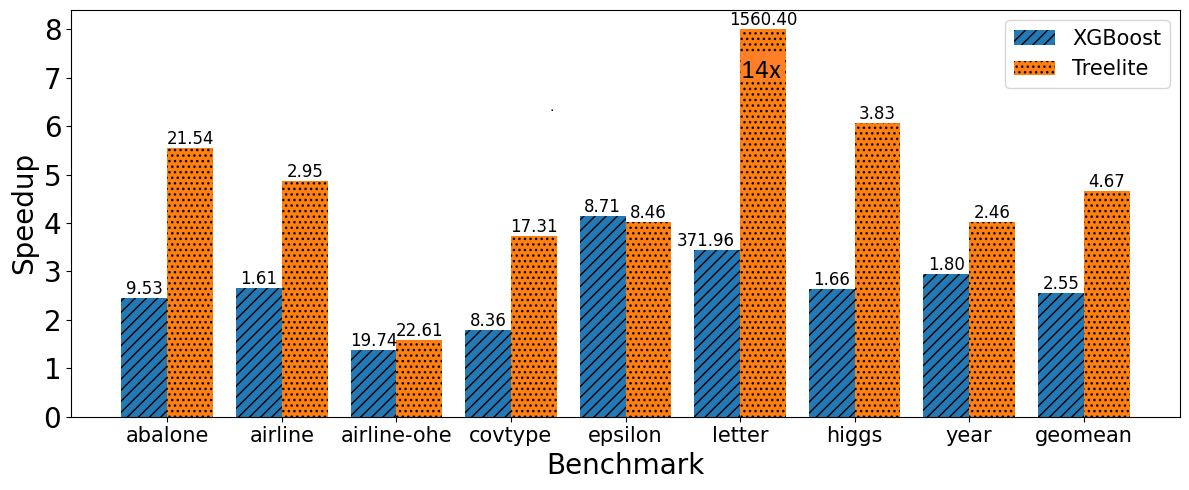
\includegraphics[width=\linewidth]{figures/result/serial_speedup_per_benchmark_xgoost_treelite.png}
%   \caption{Speedup of \Treebeard{} optimized code compared to XGBoost and Treelite on single core at batch size of 1024.}
%   \label{Fig:XGBoostSerialCompare}
% \end{figure}

\begin{figure*}
  \centering
  \subfloat[Single-core]{
    \centering
    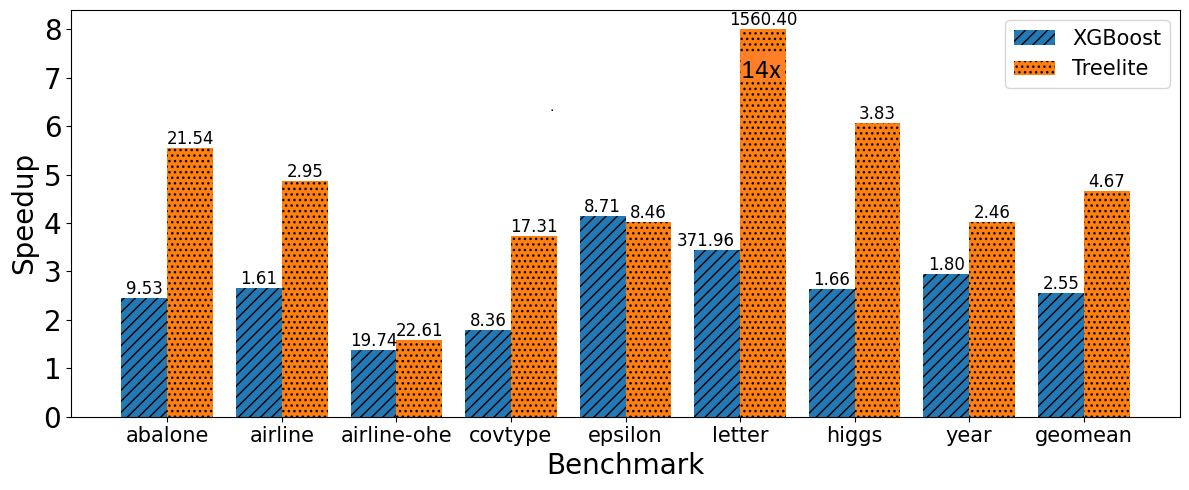
\includegraphics[width=0.48\textwidth]{figures/result/serial_speedup_per_benchmark_xgoost_treelite.png}
    \label{Fig:XGBoostSerialCompare}
  }
  \subfloat[16 cores]{
    \centering
    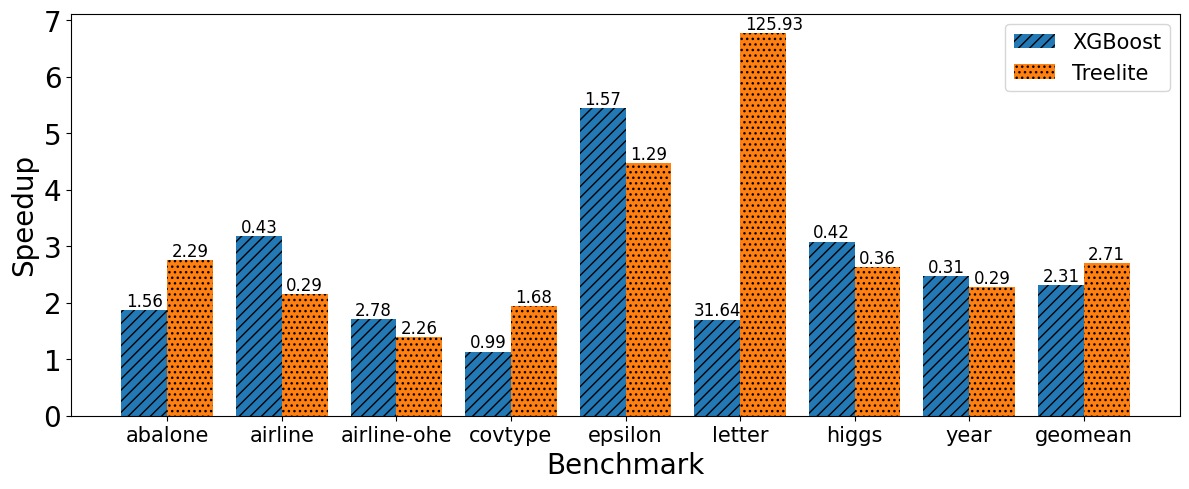
\includegraphics[width=0.48\textwidth]{figures/result/parallel_speedup_per_benchmark_xgoost_treelite.png}
    \label{Fig:XGBoostParallelCompare}
  }
  \caption{Comparison of \Treebeard{} with XGBoost and Treelite with batch size 1024. Bars show speedup of 
           \Treebeard{} optimized code relative to XGBoost and Treelite. Numbers on XGBoost speedup bars are the 
           mean inference time per row for XGBoost in $\mu$s. Numbers on the Treelite bars are mean inference times 
           for Treelite. Numbers on the geomean bars are the geomean speedups over all benchmarks.}
  \label{fig:XGBoostCompare}
\end{figure*}

\begin{figure}[tbp]
  \centering
  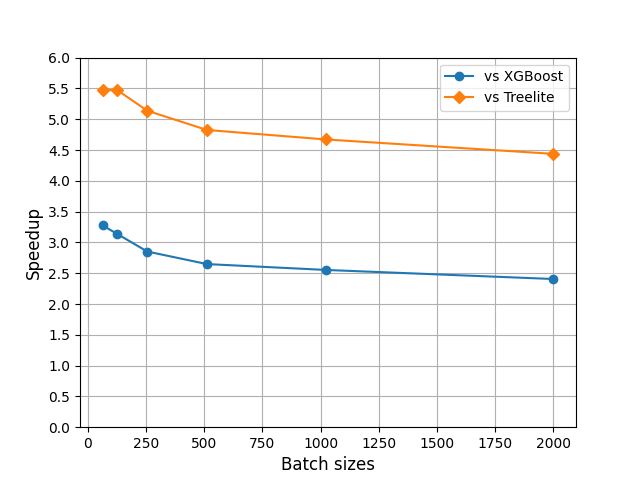
\includegraphics[width=0.8\linewidth]{figures/result/scalar_Intel_mean_speedups_treebeard_vs_xgboost_treelite.png}
  \caption{Geomean speedup (over all benchmarks) of \Treebeard{} over XGBoost
  and Treelite on single-core over several batch sizes.}
\label{Fig:XGBoostBatchSizeCompare} \end{figure}

Figures~\ref{Fig:XGBoostSerialCompare} and~\ref{Fig:XGBoostParallelCompare} report a comparison of \Treebeard{} with
two state-of-the-art frameworks, XGBoost~\cite{XGBoost} which is widely used by ML practitioners and Treelite~\cite{Treelite} a
basic compiler for decision tree inference. As the plots show, \Treebeard{} is significantly better than both these systems.
It is atleast $2\times$ faster on most benchmarks over either systems in both single-core and multi-core settings.
Figure~\ref{Fig:XGBoostBatchSizeCompare} shows that these performance improvements are consistent across a wide range of input batch sizes. 
\Treebeard{} performs several novel optimizations that neither of these systems perform. In fact, apart from parallelization,
all the other optimizations (tiling, tree-ordering, walk interleaving, walk peeling, vectorization and layout optimizations)
in \Treebeard{} are new. These results demonstrate the utility of building a generic compiler to implement different optimizations.


\subsection{Sensitivity Analysis}
This section reports the impact of individual optimizations and reports the sensitivity of results to both batch size and degree of parallelism. All speedup's are with respect to the scalar baseline running on a single core.
\subsubsection{Impact of Optimizations}

\begin{figure*}
  \centering
  \subfloat[Tiling]{
    \centering
    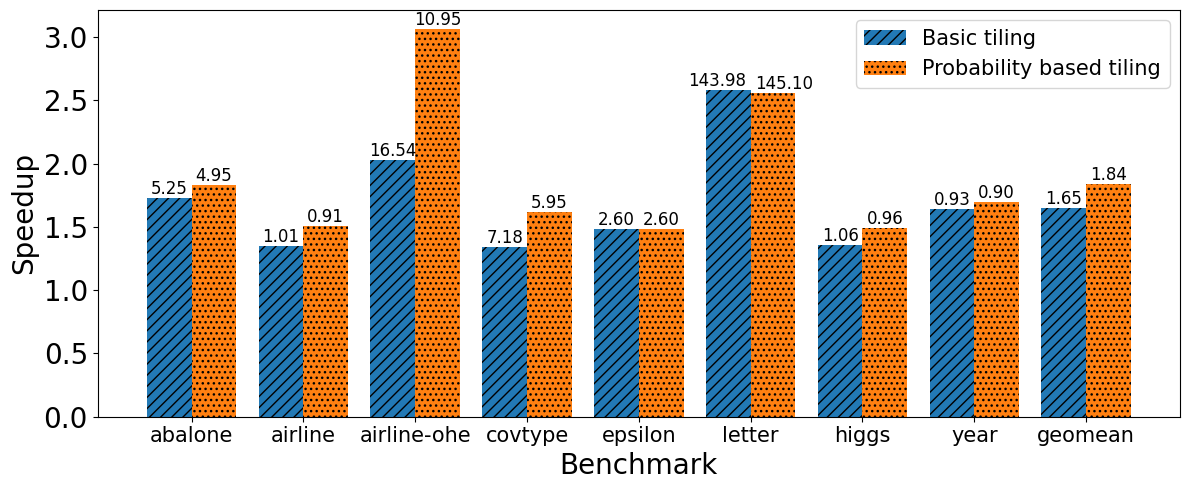
\includegraphics[width=0.48\linewidth]{figures/result/scalar_Intel_max_speedup_unif_prob_tiling.png}
    \label{Fig:IntelTiling1024}
    }
  \subfloat[Walk Unrolling, Walk Interleaving]{
    \centering
    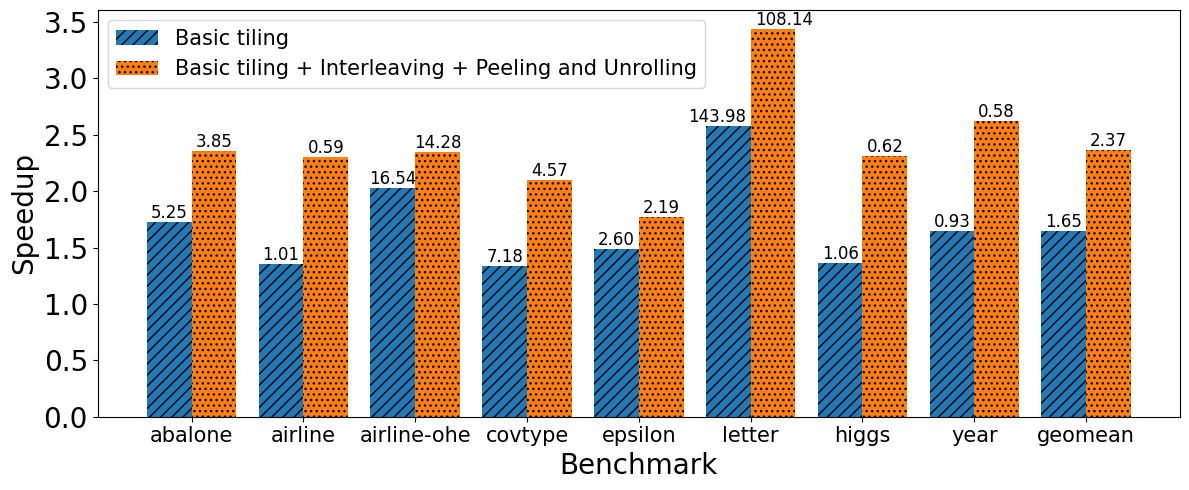
\includegraphics[width=0.48\linewidth]{figures/result/scalar_Intel_max_speedup_unif_tiling_pipelining.png}
    \label{Fig:IntelInterleaving1024}
    }
  \caption{Impact of individual \Treebeard{} optimizations at batch size 1024 (Intel RocketLake).
           Number on the bar is the average inference time per row in $\mu$s. Numbers on the geomean bars are the geomean
           speedups over all benchmarks.}
  \label{fig:OptSpeedup}
\end{figure*}


Figure~\ref{Fig:IntelTiling1024} compares different tiling algorithms on Intel (the trends on AMD are identical,
though as explained before the best tile sizes differ), the plot has two bars per benchmarks one shows the speedup
over baseline when all trees use the basic tiling algorithm, while the second tiles leaf-biased trees
($\langle\alpha =0.075, \beta =0.9 \rangle$ as defined in Section~\ref{sec:ProbTiling})  with probability-based tiling
(other trees continue to be tiled with basic tilling). The number of leaf-biased trees in each model 
is given in the last column of Table~\ref{Tab:Benchmarks}. For these plots we disable all mid-level IR optimizations,
but apply the low level optimizations as they go hand-in-hand with tiling.

As can be seen, even basic tiling is highly efficient, speeding up benchmarks by $1.3 - 2.5\times$.
Probability-based tilling does even better. Recall that probability-based tiling makes use of additional information about leaf probabilities (how
often a particular leaf is encountered while performing inference on the training data). As seen from the graph,
specializing the tiling to this property of the model yields additional gains. The speedup increases from
$2\times$ to $3.1\times$ for \op{airline-ohe}, the benchmark with the highest fraction of leaf-biased trees.
Several other benchmarks see an increase in speedup of $0.2- 0.4\times$. Three benchmarks~\op{epsilon, year}
and \op{letter} see little or no impact because these benchmarks have no leaf-biased trees.

Figure~\ref{Fig:IntelInterleaving1024} shows the additional benefit over and above tiling 
that \op{tree walk interleaving} and \op{tree walk peeling \& unrolling} achieve.
As can be seen these optimizations bring in significant additional improvements (on average the speedup improves from $1.5\times$ to $2.4\times$).
As discussed earlier these optimizations target different bottlenecks; while tiling improves locality and enables vectorization, these
optimizations eliminate different sources of pipeline stalls.
This clearly highlights the need for an extensible compiler framework where independent optimizations can be added at different levels of abstraction.

\subsubsection{Impact of Batch Size}
Figure~\ref{Fig:OverallScalarOverBatchSizes} shows the geomean speedup over all benchmarks for various batch size when all \Treebeard{} optimizations
are performed. The graph shows that the speedups due to \Treebeard{}'s 
optimizations work equally well across all batch sizes on both the Intel and the 
AMD machines. We infer that it would be useful to specialize tiling over the 
batch size to the target machine from the slightly different trends for the 
Intel and AMD machines. However, we leave this for future work.  
We also find that performance of \Treebeard{}'s generated 
code scales well with an increasing number of cores (plot not shown). Even though \Treebeard{} 
currently only implements a na\"ive parallelization strategy, performance scales 
reasonably well with increasing number of cores.

Overall, our results show that \Treebeard{} provides significant performance gains compared to existing systems like XGBoost and Treelite.
The optimizations designed and implemented in \Treebeard{} provide significant speedups. Also, these speedups are robust to changes
in hardware and parameters like batch size.

% \begin{figure}[htbp]
%   \centering
%   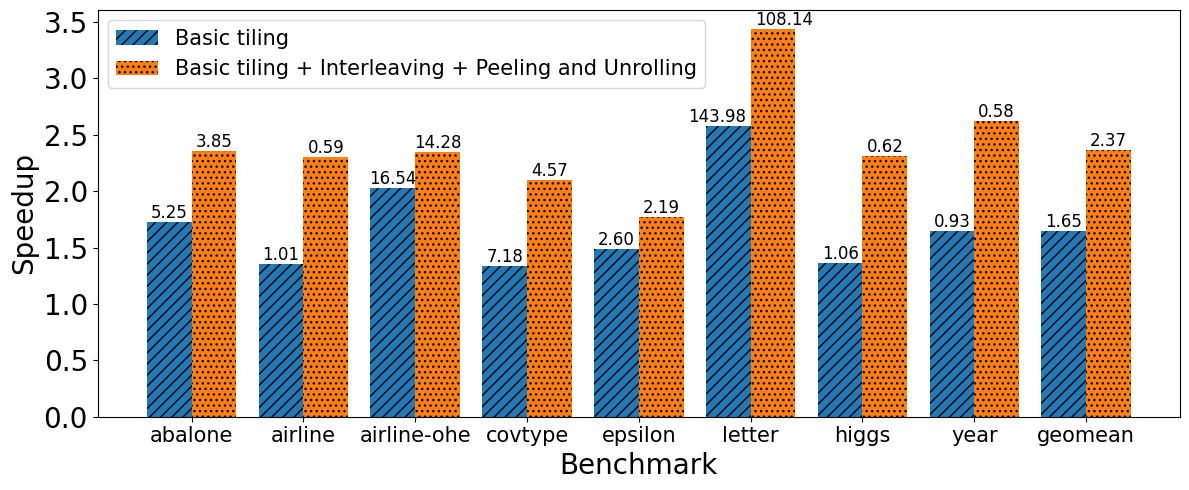
\includegraphics[width=0.8\linewidth]{figures/result/scalar_Intel_max_speedup_unif_tiling_pipelining.png}
%   \caption{Speedups (single core) due to walk unrolling and walk interleaving at batch size 1024 (Intel RocketLake).
%            Number on the bar is the average inference time per row in $\mu$s. Numbers on the geomean bar are 
%            the geomean speedups over all benchmarks. }
%   \label{Fig:IntelInterleaving1024}
% \end{figure}

\begin{figure}[htbp]
  \centering
  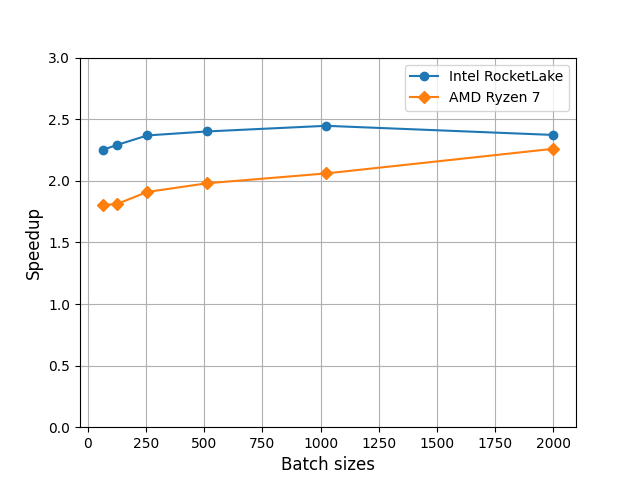
\includegraphics[width=0.8\linewidth]{figures/result/scalar_overall_mean_speedups_intel_amd.png}
  \caption{Geomean speedup (over all benchmarks) of optimized \Treebeard{} code over the scalar baseline on single-core
           over several batch sizes.}
  \label{Fig:OverallScalarOverBatchSizes}
\end{figure}

% \begin{figure}
%   \centering
%   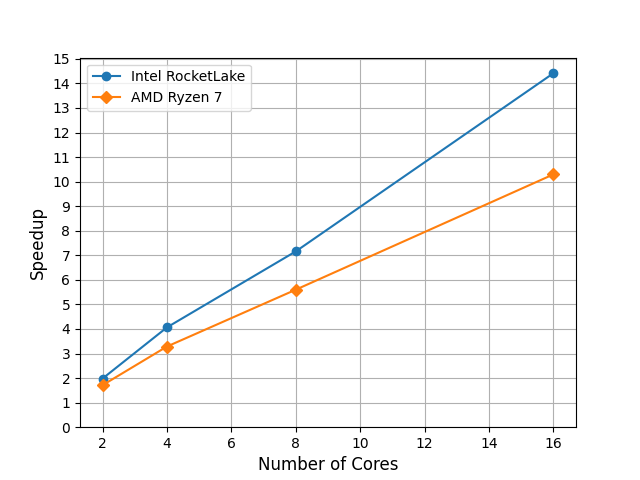
\includegraphics[width=\linewidth]{figures/result/parallel_core_scaling_intel_amd.png}
%   \caption{\Treebeard{} scaling with varying number of cores. Speedup is computed over the na\"ive \Treebeard{} scalar baseline.}
%   \label{Fig:CoreScaling}
% \end{figure}
